%% Submissions for peer-review must enable line-numbering 
%% using the lineno option in the \documentclass command.
%%
%% Camera-ready submissions do not need line numbers, and
%% should have this option removed.
%%
%% Please note that the line numbering option requires
%% version 1.1 or newer of the wlpeerj.cls file, and
%% the corresponding author info requires v1.2

\documentclass[lineno]{wlpeerj}
\usepackage[utf8]{inputenc}
\usepackage[T1]{fontenc}
\usepackage{hyperref}
\usepackage{url}
\usepackage{booktabs}
\usepackage{amsmath}
\usepackage{amsfonts}
\usepackage{microtype}
\usepackage{graphicx}
% preamble
\usepackage{tikz}
\usetikzlibrary{arrows.meta, positioning}


\begin{document}
	\title{Extending Neural Networks: Lateral Propagation and Multimodal Convolution}
	
	\author{
		Jay Kumar \\
		Independent Researcher \\
		Austin, TX \\
		\texttt{j.kumar.nbl@gmail.com}
	}
	
	
	\begin{abstract}
		
		Neural network architectures have traditionally evolved along two largely independent axes: improvements in learning mechanisms and improvements in representational capacity. Recurrent neural networks rely on backpropagation through time (BPTT) to model temporal dependencies, while convolutional neural networks (CNNs) exploit spatial locality and are primarily applied to visual domains.
		
		In this work, we decouple these dimensions and investigate two orthogonal extensions. First, we introduce a persistent-memory sequence model that replaces BPTT with localized updates and lateral propagation. Second, we demonstrate that convolution can be extended beyond visual domains to multimodal structured data.
		
	Experimental results show that localized propagation captures training-set structure but fails to generalize under the tested single-modal configuration, while multimodal convolution improves held-out classification performance as data scale increases. Although limitations remain, these results suggest that neural architectures can be redesigned at a higher level of abstraction by independently modifying learning and representation mechanisms.
	\end{abstract}
	
	
	\flushbottom
	
	\maketitle
	%%	\keywords Convolutional Neural Networks \And Lateral Propagation \And Multimodal Learning \And Persistent Memory
	
	\thispagestyle{empty}
	\section{Introduction}
	Recurrent neural networks (RNNs) and convolutional neural networks (CNNs) represent two foundational paradigms in modern machine learning \cite{goodfellow2016deep, lecun1998gradient}. Despite their success, both architectures are constrained by specific design assumptions.
	
	RNNs rely on backpropagation through time (BPTT), which introduces significant computational overhead and limits scalability. CNNs, while highly effective, are typically treated as domain-specific architectures for visual data.
	
	In this work, we argue that these architectures can be understood at a higher level of abstraction. Specifically, we treat:
	
	\begin{itemize}
		\item Learning mechanisms (e.g., backpropagation vs localized updates)
		\item Representation strategies (e.g., unimodal vs multimodal convolution)
	\end{itemize}
	
	as independent design dimensions.
	
	We explore two corresponding extensions:
	
	\begin{enumerate}
		\item A persistent-memory sequence model that replaces BPTT with localized lateral propagation
		\item A multimodal convolutional framework that generalizes CNNs beyond visual domains
	\end{enumerate}
	
	Together, these contributions suggest that neural architectures can be extended by decoupling learning dynamics from representational structure.
	
	\section{Background}
	
	Traditional RNNs propagate information through hidden states and optimize parameters via gradient descent across time steps. While effective, this approach suffers from vanishing gradients and high computational cost.
	
	Early neural models such as the perceptron \cite{rosenblatt1958perceptron} and connectionist frameworks \cite{rumelhart1986pdp} established the basis for distributed learning. Hebbian learning \cite{hebb1949organization} further motivates localized update rules.
	
	CNNs address structured learning by exploiting locality through shared weights and hierarchical feature extraction \cite{lecun1998gradient}. However, their application has remained largely restricted to visual data.
	
	Recent architectures such as transformers aim to address these limitations but often introduce substantial computational overhead.
	
	\section{Materials and Methods}
	
	\subsection{Persistent-Memory Sequence Model}
	
	We propose a sequence learning model that replaces BPTT with localized updates using persistent memory structures.
	
	The model consists of:
	
	\begin{itemize}
		\item \textbf{Node Memory}: Stores token-position relationships conditioned on class labels
		\item \textbf{Lateral Memory}: Stores token-to-token transitions
		\item \textbf{Class Statistics}: Tracks class frequency for normalization
	\end{itemize}
	
	Training occurs through incremental updates to these structures. During inference, class scores are computed as:
	
	\begin{equation}
		S(c) = \alpha \cdot M_{pos}(c) + \beta \cdot M_{lat}(c) + \gamma \cdot F(c)
	\end{equation}
	
	where:
	\begin{itemize}
		\item $M_{pos}$ represents positional matches
		\item $M_{lat}$ represents lateral transitions
		\item $F(c)$ is the class frequency normalization
	\end{itemize}
	
	This formulation replaces global gradient propagation with localized accumulation and inference.
	
	\subsection{Multimodal Convolution}
	
	We extend convolutional architectures to multimodal structured data.
	
	Each modality (e.g., visual frames, audio spectrograms) is processed through an independent convolutional pathway. These representations are then fused at a higher level.
	
	This approach reframes convolution as a general mechanism for learning localized structure rather than a vision-specific technique.
	\subsection{Dataset}
	
	Experiments were conducted using the Human Activity Recognition Video Dataset from Kaggle \cite{dataset}, available at \url{https://www.kaggle.com/dsv/5722068} and DOI \url{https://doi.org/10.34740/KAGGLE/DSV/5722068}. The dataset consists of labeled video samples across multiple activity classes and contains approximately 15 GB of video data organized into class-specific directories.
	
	
\subsection{Data Preprocessing}

Videos were split into training and testing sets using an 80/20 split. To evaluate the effect of data scale, training subsets of size 500, 1000, and 1500 were requested. However, the effective training size was bounded by the available data after splitting, resulting in a maximum usable training size of 890 samples.

The reduction in effective training size is due to class-balanced sampling and dataset partitioning constraints.

Each video was processed into two synchronized modalities: visual frames and audio. For the visual modality, each video was uniformly sampled into $T$ RGB frames, resized to $128 \times 128$, and normalized to $[0,1]$. For the audio modality, the audio stream was extracted at 16 kHz, converted into a log-spectrogram, and resized to $128 \times 128$.

\subsection{Multimodal CNN Architecture}

Each sampled RGB frame was passed through a convolutional branch consisting of four convolutional blocks with batch normalization, ReLU activations, pooling, and adaptive average pooling. The resulting per-frame embeddings were averaged across time to produce a single visual representation.

The audio spectrogram was passed through an independent convolutional branch. This branch produced an audio embedding of the same dimensionality as the visual embedding.

The two modality embeddings were concatenated and passed through a fully connected classifier:

\begin{equation}
	z_v = f_v(X_v), \qquad z_a = f_a(X_a)
\end{equation}

\begin{equation}
	z = [z_v ; z_a]
\end{equation}

\begin{equation}
	\hat{y} = \mathrm{softmax}(g(z))
\end{equation}

where $X_v$ denotes the sampled video frames, $X_a$ denotes the audio spectrogram, $f_v$ and $f_a$ are the visual and audio convolutional branches, and $g$ is the final multilayer classifier.

\begin{figure}[t]
	\centering
	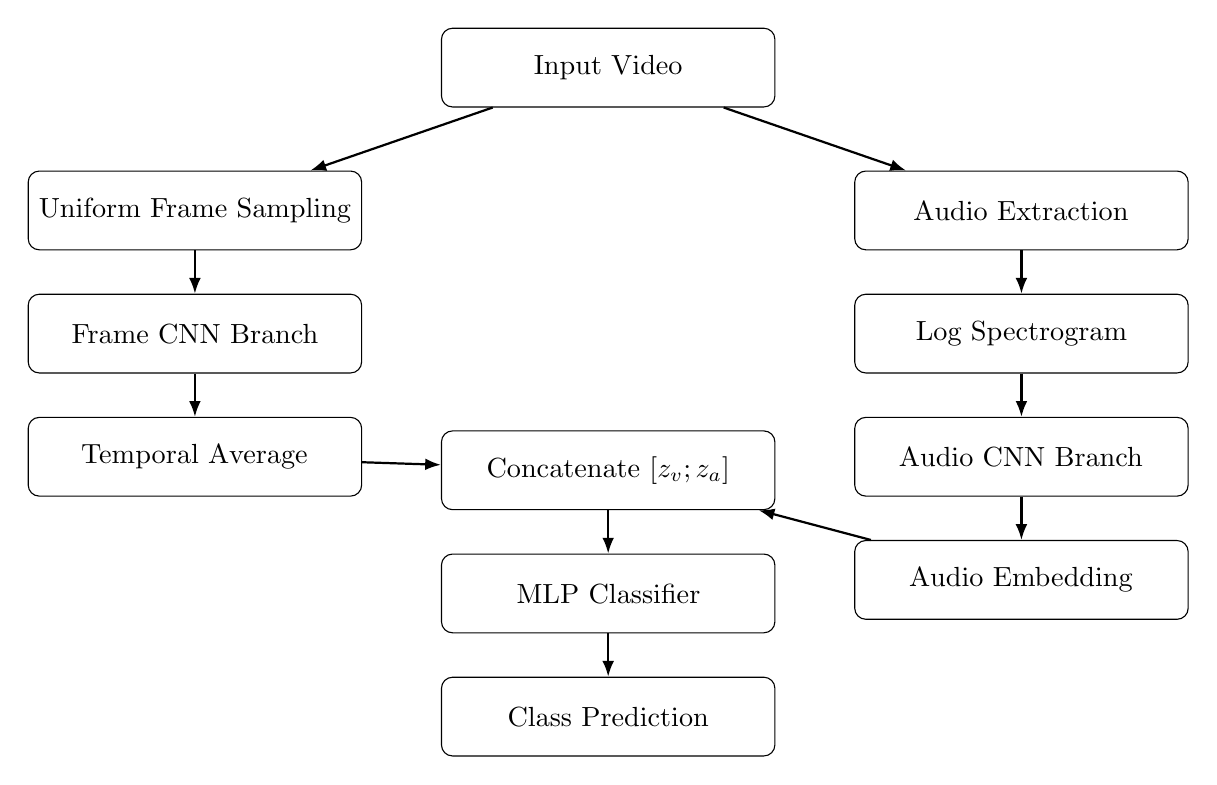
\begin{tikzpicture}[
		node distance=0.55cm,
		block/.style={
			draw,
			rounded corners,
			align=center,
			text width=4cm,
			minimum height=1cm,
			font=\normalsize
		},
		arrow/.style={-{Latex[length=2mm]}, thick}
		]
		
		\node[block] (video) {Input Video};
		
		\node[block, below left=0.8cm and 1.0cm of video] (frames)
		{Uniform Frame Sampling};
		
		\node[block, below=of frames] (framecnn)
		{Frame CNN Branch};
		
		\node[block, below=of framecnn] (frameavg)
		{Temporal Average};
		
		\node[block, below right=0.8cm and 1.0cm of video] (audio)
		{Audio Extraction};
		
		\node[block, below=of audio] (spec)
		{Log Spectrogram};
		
		\node[block, below=of spec] (audiocnn)
		{Audio CNN Branch};
		
		\node[block, below=of audiocnn] (audioemb)
		{Audio Embedding};
		
		\node[block, below=4.1cm of video] (concat)
		{Concatenate $[z_v;z_a]$};
		
		\node[block, below=of concat] (mlp)
		{MLP Classifier};
		
		\node[block, below=of mlp] (pred)
		{Class Prediction};
		
		\draw[arrow] (video) -- (frames);
		\draw[arrow] (frames) -- (framecnn);
		\draw[arrow] (framecnn) -- (frameavg);
		\draw[arrow] (frameavg) -- (concat);
		
		\draw[arrow] (video) -- (audio);
		\draw[arrow] (audio) -- (spec);
		\draw[arrow] (spec) -- (audiocnn);
		\draw[arrow] (audiocnn) -- (audioemb);
		\draw[arrow] (audioemb) -- (concat);
		
		\draw[arrow] (concat) -- (mlp);
		\draw[arrow] (mlp) -- (pred);
		
	\end{tikzpicture}
	\caption{Multimodal CNN architecture. Each video is represented using sampled RGB frames and an audio-derived log-spectrogram. Independent convolutional branches produce modality-specific embeddings, which are concatenated and classified using a multilayer perceptron.}
	\label{fig:multimodal-cnn}
\end{figure}

\subsection{Training Procedure}

The multimodal CNN was trained using the Adam optimizer with a learning rate of $10^{-3}$ and weight decay of $10^{-4}$. Models were trained for 5 epochs with a batch size of 8. Cross-entropy loss was used for optimization. All experiments were implemented in PyTorch.

\subsection{Evaluation Method}

The proposed approaches were evaluated using supervised classification experiments. Training data were used to fit or update each model, while held-out test data were used only for evaluation.

The persistent-memory sequence model was evaluated by measuring classification performance after localized updates to node memory, lateral memory, and class statistics. This evaluation was used to determine whether persistent memory and lateral propagation could support classification without backpropagation through time.

The multimodal CNN was evaluated using the same held-out testing procedure. This evaluation measured whether multimodal convolution improved generalization as the amount of available training data increased.
	
\subsection{Assessment Metrics}

Model performance was assessed using training accuracy and test accuracy. Training accuracy measures the proportion of correctly classified samples in the training set and was used to evaluate whether the model captured structure present in the training data. Test accuracy measures the proportion of correctly classified samples in the held-out test set and was used to estimate generalization performance on unseen data.

For the persistent-memory sequence model, the difference between training accuracy and test accuracy was used to assess whether localized propagation produced transferable representations or primarily memorized training structure. For the multimodal CNN, changes in test accuracy across training sizes were used to evaluate whether additional data improved generalization.
	
\subsection{Reproducibility Materials}

Code, experiment instructions, dataset source information, requirements, and reproduction notes are provided in the accompanying GitHub repository: \url{https://github.com/kenseitehdev/Extending-Neural-Networks-Lateral-Propagation-and-Multimodal-Convolution.git}. The repository includes a README file describing the project, dataset, code organization, usage instructions, software requirements, methodology, citations, and licensing information.
	
	The following section evaluates both proposed approaches under the experimental setup described above.
	
\section{Results}

\subsection{Single-Modal Lateral-Propagation Baseline}

The single-modal lateral-propagation configuration achieved an average training accuracy of 66.1\%, indicating that the model captured structure within the training data. However, held-out test accuracy remained 0.0\% across all evaluated sample sizes. This suggests that the tested single-modal configuration did not generalize beyond the training set and requires further refinement before it can support robust classification.

	\begin{table}[h]
	\centering
	\begin{tabular}{lccc}
		\toprule
		Metric & 500 Samples & 1000 Samples & 1500 Samples \\
		\midrule
		Train Accuracy & 0.668 & 0.670 & 0.646 \\
		Test Accuracy & 0.000 & 0.000 & 0.000 \\
		\bottomrule
	\end{tabular}
\caption{Single-modal lateral-propagation baseline performance.}
\end{table}


\subsection{Multimodal Convolution}


The multimodal CNN achieved stronger held-out performance than the single-modal configuration. Across the evaluated runs, the multimodal model produced an average training accuracy of 52.8\% and an average test accuracy of 52.5\%. At the maximum usable training size of 890 samples, test accuracy increased to 63.7\%, indicating that the fused visual-audio representation improved generalization under the tested configuration.

These results suggest that multimodal fusion provided useful information beyond the single-modal configuration. The improvement should be interpreted within the limits of the experimental setup, since additional single-modal baselines, longer training schedules, and alternative preprocessing choices may produce different comparative results.
	
	\begin{table}[h]
		\centering
		\begin{tabular}{lcc}
			\toprule
			Metric & 500 Samples & 890 Samples \\
			\midrule
			Train Accuracy & 0.500 & 0.556 \\
			Test Accuracy & 0.413 & 0.637 \\
			\bottomrule
		\end{tabular}
		\caption{Multimodal CNN performance}
	\end{table}
	
The improvement in test accuracy suggests that convolutional branches can be applied to multiple structured modalities when those modalities preserve local relationships. In this experiment, visual frames and audio-derived spectrograms provided complementary structure that improved classification relative to the tested single-modal configuration.
	
	Notably, average prediction confidence remains relatively stable across runs, suggesting that improvements in accuracy are driven by more correct predictions rather than increased model certainty.
\section{Discussion}

\subsection{Learning Without BPTT}

The single-modal lateral-propagation configuration demonstrates that localized memory updates can capture structure within the training data without relying on backpropagation through time. However, the failure to generalize to held-out samples indicates that the current formulation is not sufficient for robust classification. This suggests that additional mechanisms, such as normalization, validation constraints, regularization, or improved memory-selection rules, are required before localized propagation can serve as a practical alternative to BPTT.

\subsection{Generalizing Convolution}

The multimodal results suggest that convolutional branches can be applied to multiple structured modalities when those modalities preserve local relationships. In this study, visual frames and audio-derived spectrograms were processed through independent convolutional pathways and fused before classification. The improvement over the single-modal configuration indicates that multimodal fusion contributed useful information under the tested conditions.

\subsection{Abstraction as a Design Principle}

These findings support the broader view that neural architectures can be modified along separable design dimensions. The lateral-propagation experiment modifies the learning mechanism by replacing global temporal gradient propagation with localized memory updates. The multimodal convolution experiment modifies representational structure by applying convolutional processing to multiple synchronized modalities. Although the two experiments differ in outcome, both support the value of treating learning dynamics and representational structure as independent architectural choices.

\subsection{Limitations}

The proposed approaches exhibit several limitations. The single-modal lateral-propagation configuration failed to generalize beyond training data under the tested setup, indicating that local propagation alone is insufficient for robust classification in its current form.

The multimodal CNN, while more effective than the tested single-modal configuration, relies on relatively simple fusion through feature concatenation. More sophisticated fusion mechanisms may better capture cross-modal interactions. The comparison is also limited by the single-modal baseline failure, since alternative single-modal configurations, longer training schedules, or different preprocessing choices may produce stronger baseline performance.

Additionally, experiments were conducted on a single dataset with a limited maximum usable training size after class-balanced sampling and partitioning. Further validation across larger datasets, additional activity-recognition benchmarks, and alternative modalities is required before broader conclusions can be drawn.
	\section{Conclusion}
	
	We presented two extensions to neural network design: localized lateral propagation for sequence learning and multimodal convolution for structured representation.
	
	While limitations remain, these results demonstrate that neural networks can be restructured at a higher level of abstraction, decoupling learning mechanisms from representation strategies.
	
	Future work will focus on improving generalization in localized propagation models and refining multimodal fusion techniques.
	
	\bibliography{references}
	
\end{document}